\section{Trigger}
\label{sect:trigger}
\subsection{Trigger Study}
\label{sect:triggerstudy}

To have the best reach, two sets of triggers are compared. Their names and run ranges are shown in 
table \ref{Tab.TriggerPaths}. The corresponding prescaled triggers which are used to find the trigger plateau are also shown.

\begin{table}[!htb]
\begin{center}
\caption{On line triggers, their references and run ranges. A logical OR between SixJet and QuadJet is used.}
\label{Tab.TriggerPaths}
\begin{tabular}{|l|l|c|}
\hline
\multicolumn{3}{|c|}{HT}\\
\hline
Trigger Path & Prescaled Trigger & Run Range \\\hline
HLT\_PFHT650\_v5 & HLT\_PFHT350\_v3 & 190650-190750\\
HLT\_PFHT650\_v6 & HLT\_PFHT350\_v4 & 191000-191400\\ 
HLT\_PFHT650\_v7 & HLT\_PFHT350\_v5 & 191500-193750\\ 
HLT\_PFHT650\_v8 & HLT\_PFHT350\_v6 & 193750-196030\\ 
HLT\_PFHT650\_v9 & HLT\_PFHT350\_v7 & 196046-196531\\ 
\hline
\multicolumn{3}{|c|}{MultiJet}\\
\hline
HLT\_SixJet45\_v1  & HLT\_SixJet35\_v1  & 190640-190740\\
HLT\_SixJet45\_v2  & HLT\_SixJet35\_v2  & 191000-196030\\
HLT\_SixJet45\_v3  & HLT\_SixJet35\_v3  & 196040-196531\\
HLT\_QuadJet80\_v1 & HLT\_QuadJet70\_v1 & 190640-190740\\
HLT\_QuadJet80\_v2 & HLT\_QuadJet70\_v2 & 191000-196030\\
HLT\_QuadJet80\_v3 & HLT\_QuadJet70\_v3 & 196040-196531\\
\hline
\end{tabular}
\end{center}
\end{table}

To take into account the statistics (the peak of the selected events by the un-prescaled trigger figure \ref{fig.TriggerPlateau} (middle)),
\begin{figure}[!htb]
\centering
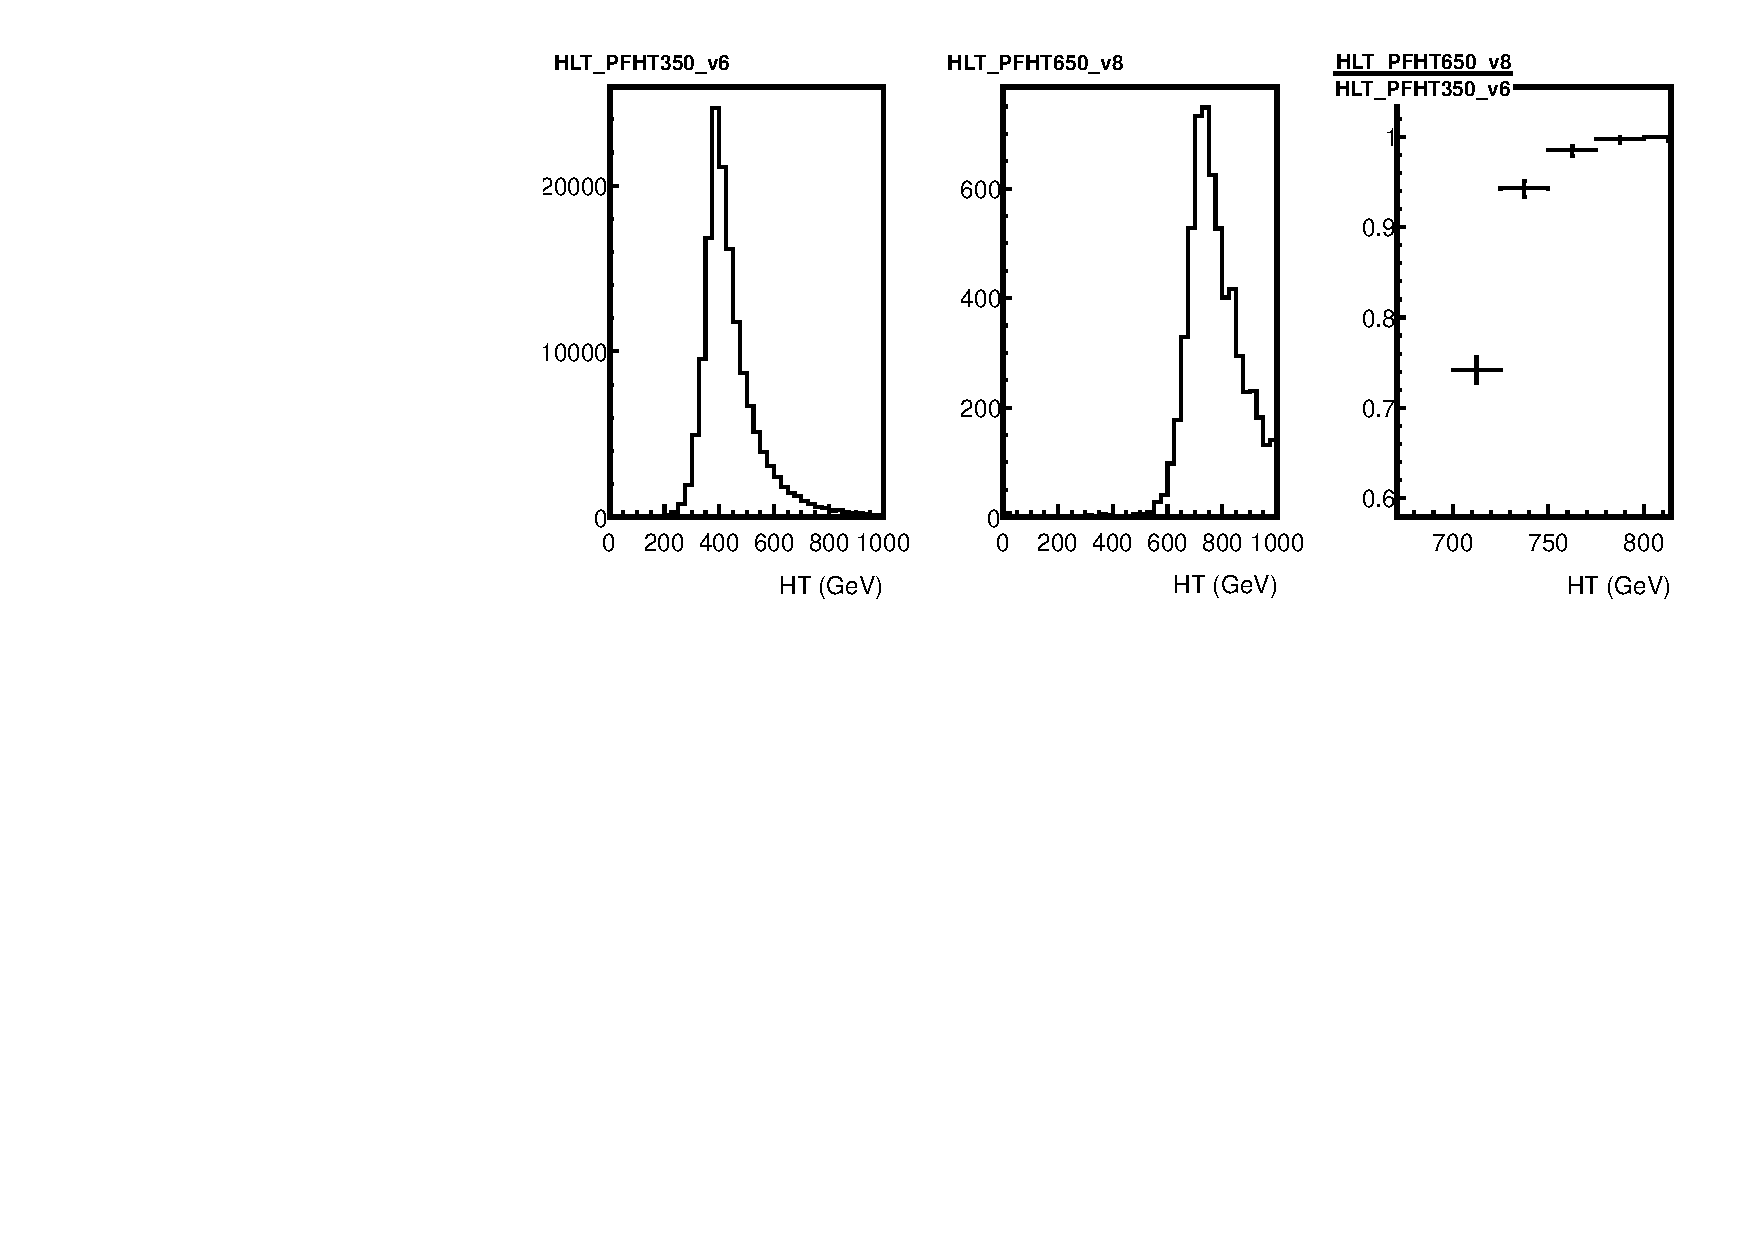
\includegraphics[width=1.0\textwidth]{figs/TriggerDemonstration.pdf}
\caption{The prescaled (left) and  un-prescaled (middle) HT triggers. The right plot shows the ratio of the two previous histograms 
zoomed in the interesting part.}
\label{fig.TriggerPlateau}
\end{figure}
we look at the efficiencies bin-by-bin and distribution of efficiencies (un-prescaled divided by the prescaled, 
figure \ref{fig.TriggerPlateau} (right)) 
with different HT cuts are weighted according to the statistics of the un-prescaled histogram. 
The cut that gives the mean value greater than 95\% is chosen as the offline cut on the trigger parameter. 
An example of this method for different cuts on the HT for HLT\_PFHT650\_vX is shown in figure \ref{fig.TriggerEff}.
\begin{figure}[!htb]
\centering
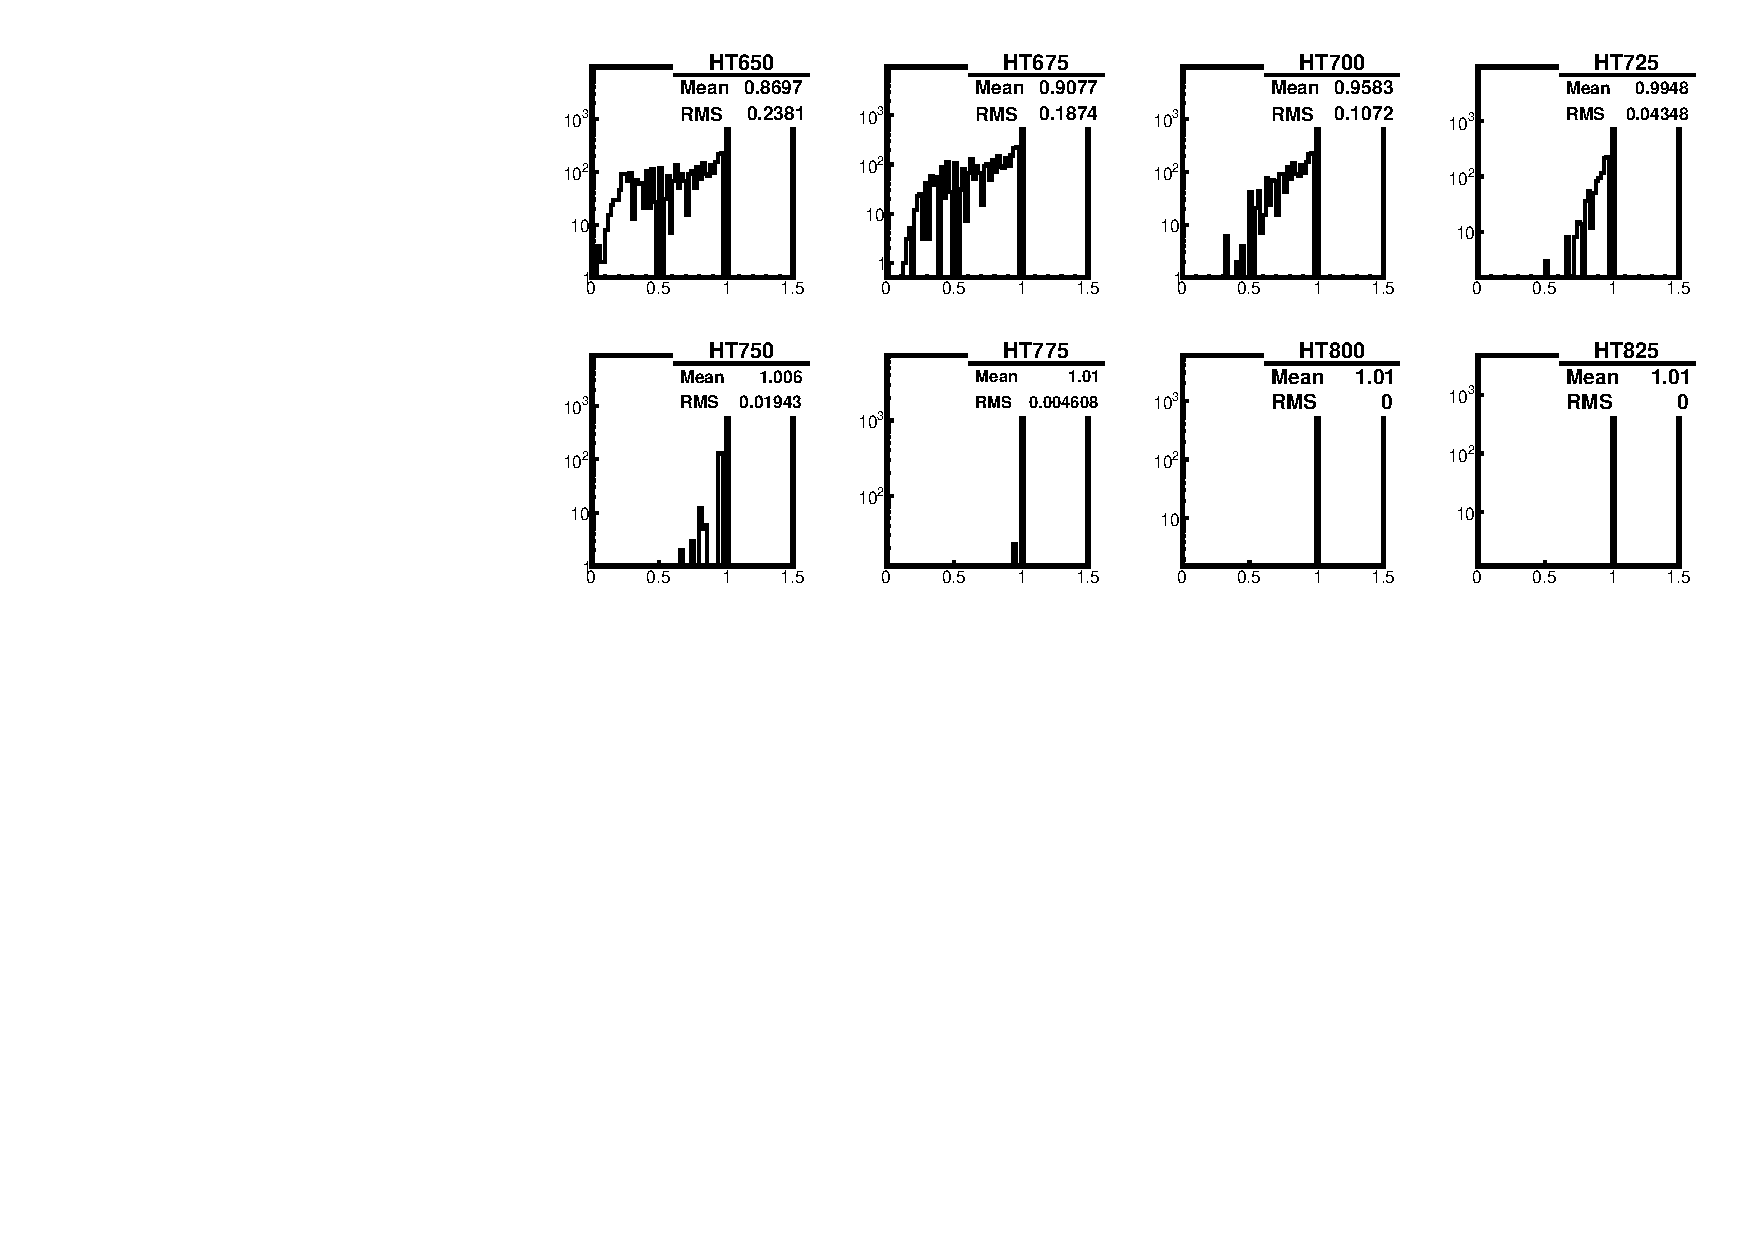
\includegraphics[width=1.0\textwidth]{figs/TriggerDemonstrationEff.pdf}
\caption{The weighted mean of the efficiencies in figure \ref{fig.TriggerPlateau}(right) for different cuts on HT. 
HT $>$ 700 GeV gives 95\% efficiency.}
\label{fig.TriggerEff}
\end{figure}

The result of this method is HT $>$ 700 GeV, but we use 725 GeV conservatively. For the multijet triggers, same method is used and 
depending on the number of jets different cuts on the  $P_T$ of the jets are found. The result is summarized here:
\begin{itemize}
\item HLT\_SixJet45\_vX, 6 jets with \pT $>$ 65 GeV/$c$ or 7 jets with \pT $>$ 55 GeV/$c$
\item HLT\_QuadJet80\_vX, 4 jets with \pT $>$ 100 GeV/$c$ or 5 jets with \pT $>$ 85 GeV/$c$
\end{itemize}
As another possibility, one can think of decreasing the number of jets and increasing the \pT threshold, but it does not reach the
plateau and is excluded from the list.

{\bf FIX ME more material and example can be added if needed!}

